\documentclass[]{ximera}
%handout:  for handout version with no solutions or instructor notes
%handout,instructornotes:  for instructor version with just problems and notes, no solutions
%noinstructornotes:  shows only problem and solutions

%% handout
%% space
%% newpage
%% numbers
%% nooutcomes

%I added the commands here so that I would't have to keep looking them up
%\newcommand{\RR}{\mathbb R}
%\renewcommand{\d}{\,d}
%\newcommand{\dd}[2][]{\frac{d #1}{d #2}}
%\renewcommand{\l}{\ell}
%\newcommand{\ddx}{\frac{d}{dx}}
%\everymath{\displaystyle}
%\newcommand{\dfn}{\textbf}
%\newcommand{\eval}[1]{\bigg[ #1 \bigg]}

%\begin{image}
%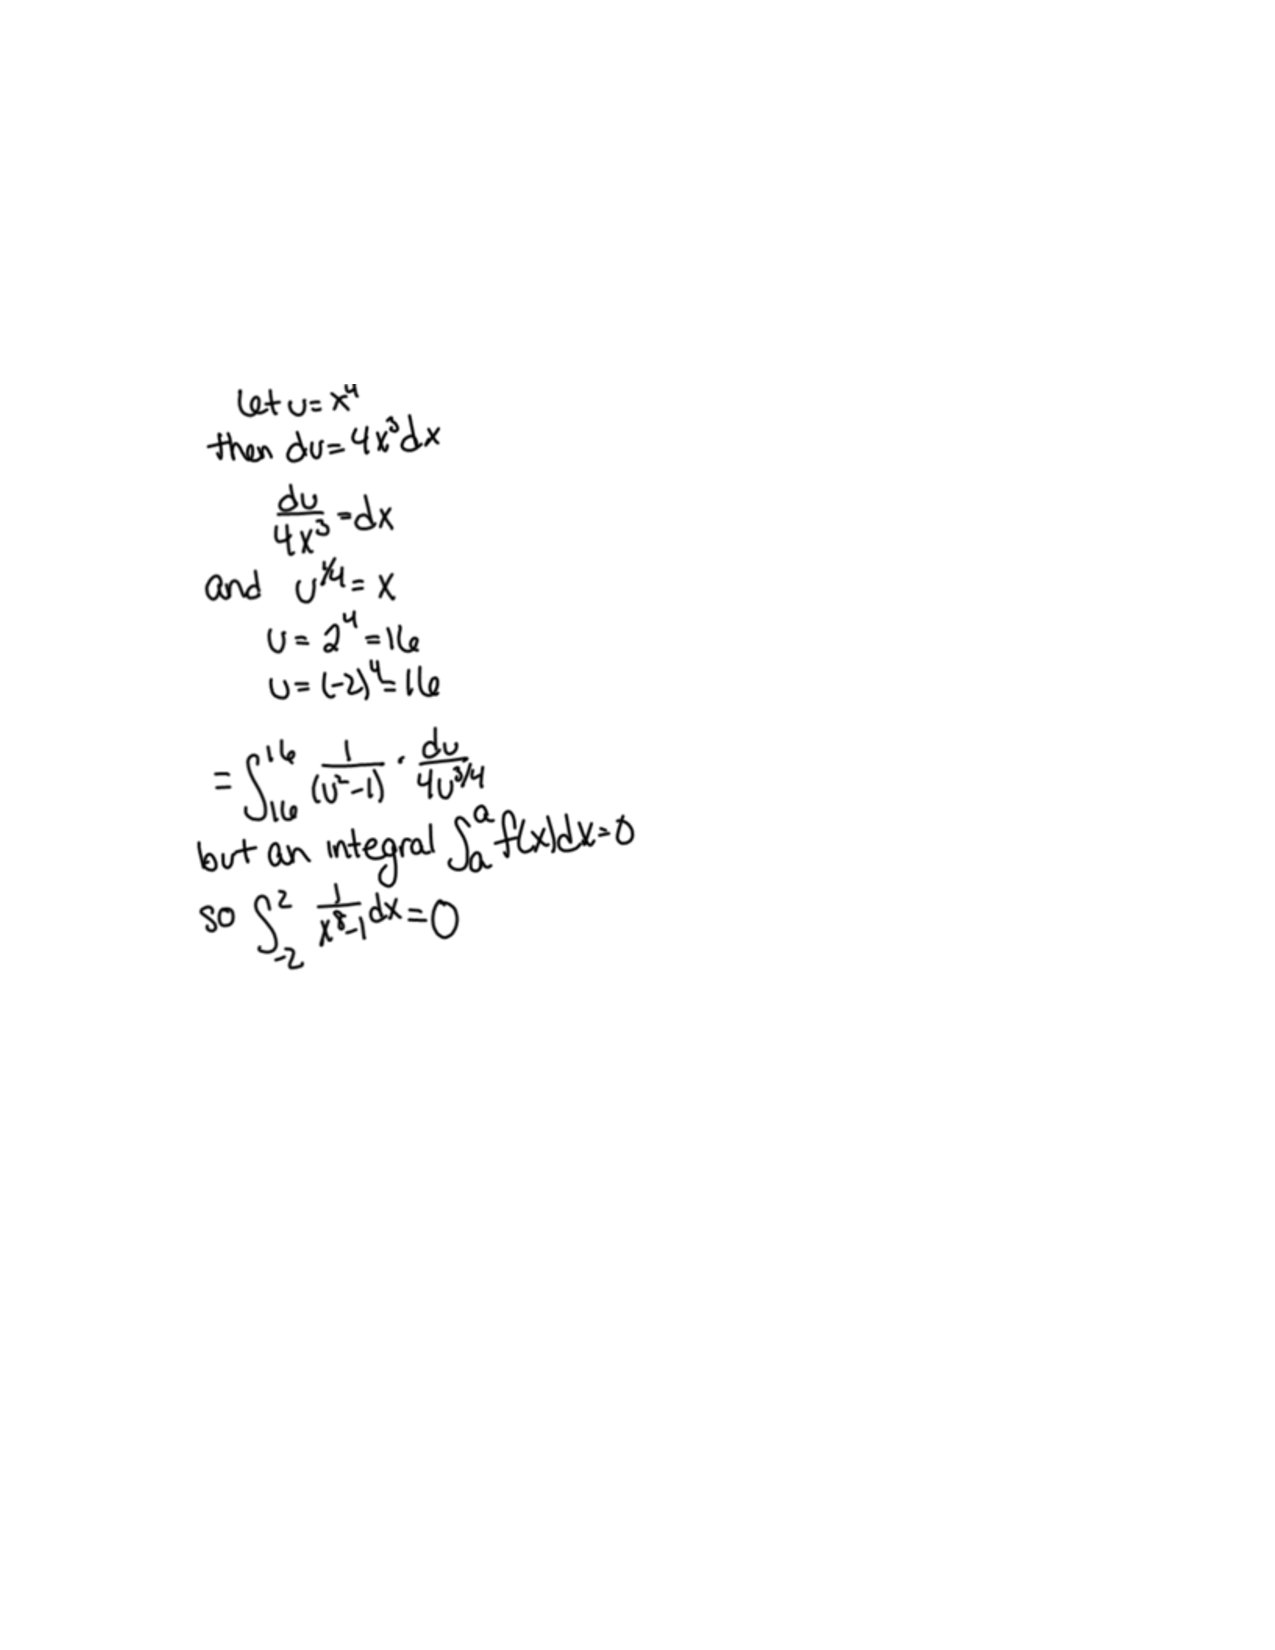
\includegraphics[trim= 170 420 250 180]{Figure1.pdf}
%\end{image}

%add a ``.'' below when used in a specific directory.
\newcommand{\RR}{\mathbb R}
\renewcommand{\d}{\,d}
\newcommand{\dd}[2][]{\frac{d #1}{d #2}}
\renewcommand{\l}{\ell}
\newcommand{\ddx}{\frac{d}{dx}}
\newcommand{\dfn}{\textbf}
\newcommand{\eval}[1]{\bigg[ #1 \bigg]}

\usepackage{multicol}

\renewenvironment{freeResponse}{
\ifhandout\setbox0\vbox\bgroup\else
\begin{trivlist}\item[\hskip \labelsep\bfseries Solution:\hspace{2ex}]
\fi}
{\ifhandout\egroup\else
\end{trivlist}
\fi} %% we can turn off input when making a master document

\title{Volume by shells}  

\begin{document}
\begin{abstract}		\end{abstract}
\maketitle



\begin{comment}
\section{Warm up:}

	\begin{freeResponse}
	
	\end{freeResponse}
	
\begin{instructorNotes}

\end{instructorNotes}
\end{comment}







\section{Group work:}



%problem 1
\begin{problem}
Set up an integral that will compute the volume of the solid generated by revolving the region bounded by the curves $y=x^2-6x+13$ (i.e. $x = 3 \pm \sqrt{y-4}$) and $y=3x-1$ about:

\begin{image}
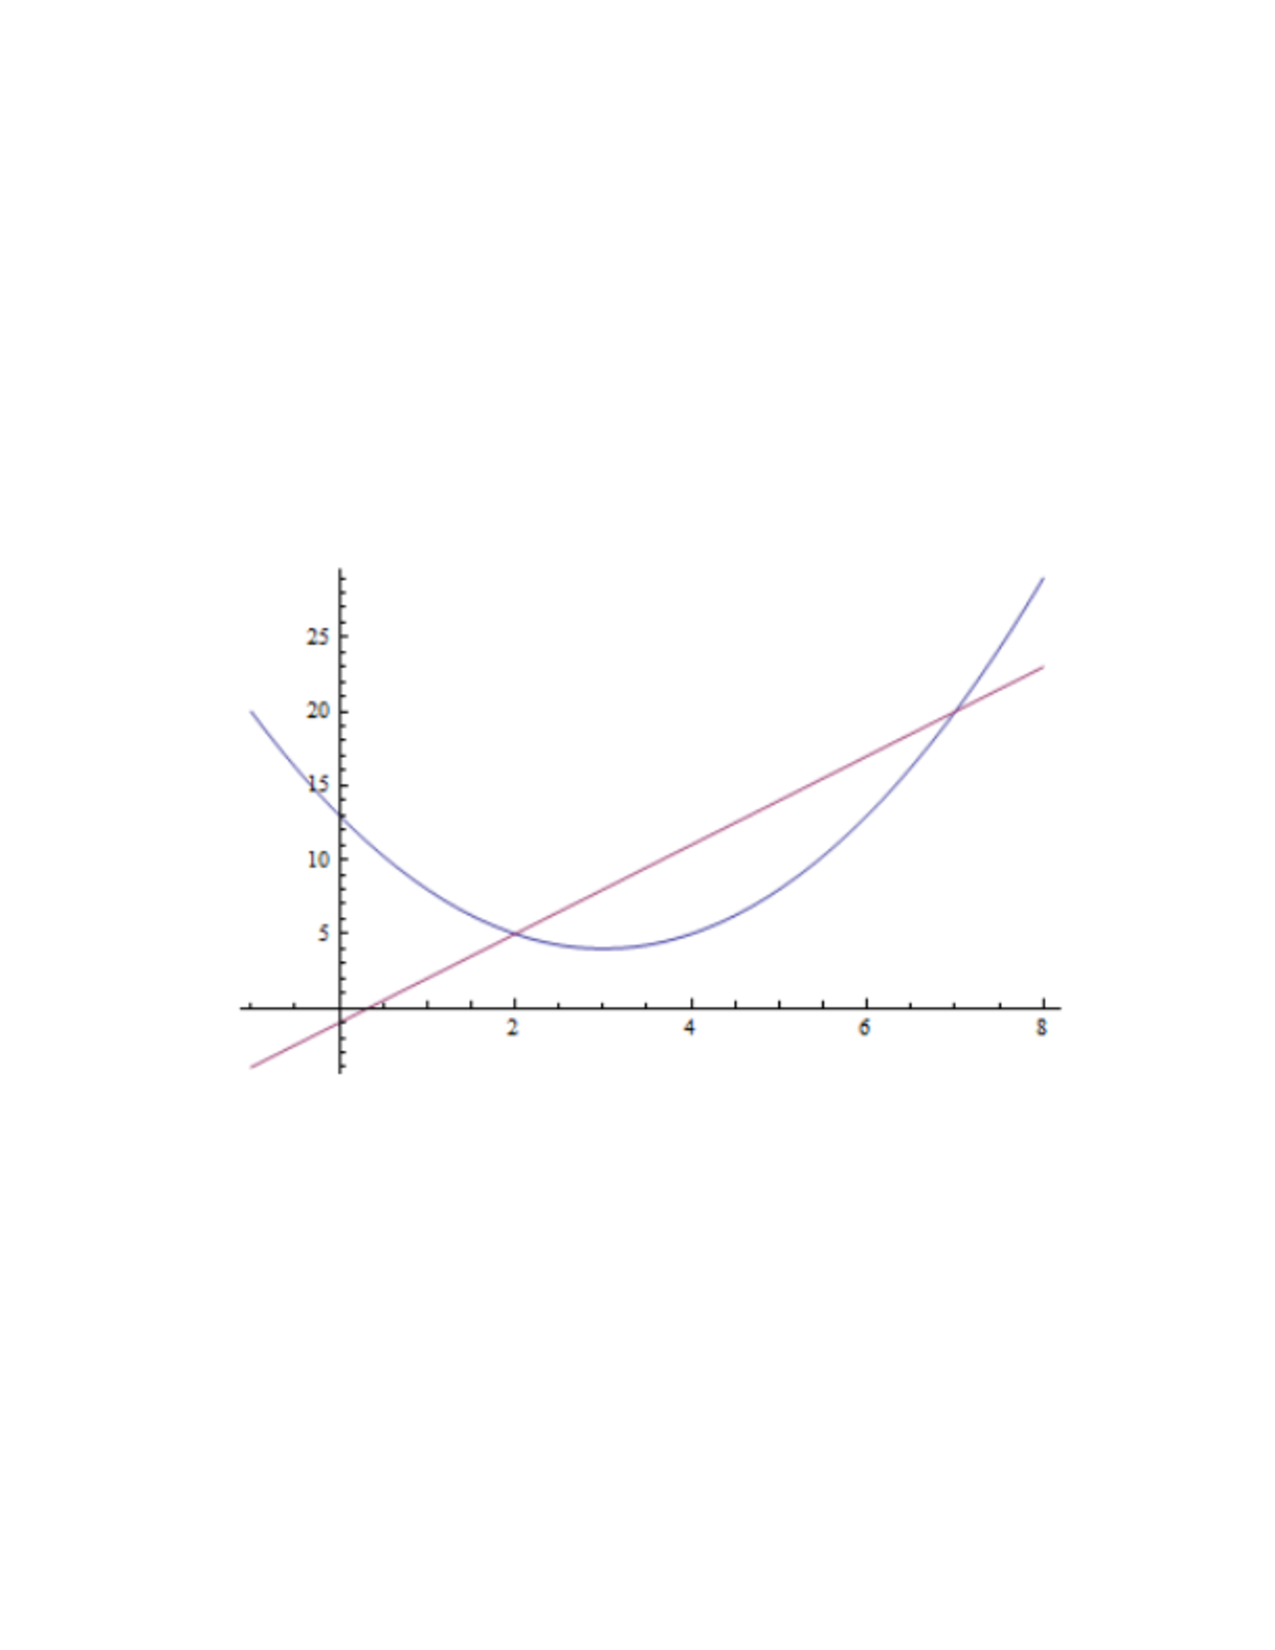
\includegraphics[trim= 170 270 150 280, scale=0.8]{Figure6-4-1.pdf}
\end{image}

	\begin{enumerate}
		\item  the $x$-axis
		\begin{freeResponse}
		First, we need to find the points where the curves intersect
			\begin{align*}
			x^2 - 6x + 13 &= 3x - 1  \\
			x^2 - 9x + 14 &= 0  \\
			(x-2)(x-7) &= 0  \\
			x &= 2, 7  \\
			(2,5&), (7,20).
			\end{align*}
		As we will see later, we also need to locate the vertex of the parabola $x^2 - 6x + 13$.  
		So we complete the square
			\begin{align*}
			y &= x^2 - 6x + 13  \\
			&= (x^2 - 6x \, {\color{red} + \, 9}) + 13 \, {\color{red} - \, 9}  \\
			&= (x-3)^2 + 4.
			\end{align*}
		So the vertex of the parabola is $(3,4)$.  
		
		\begin{image}
		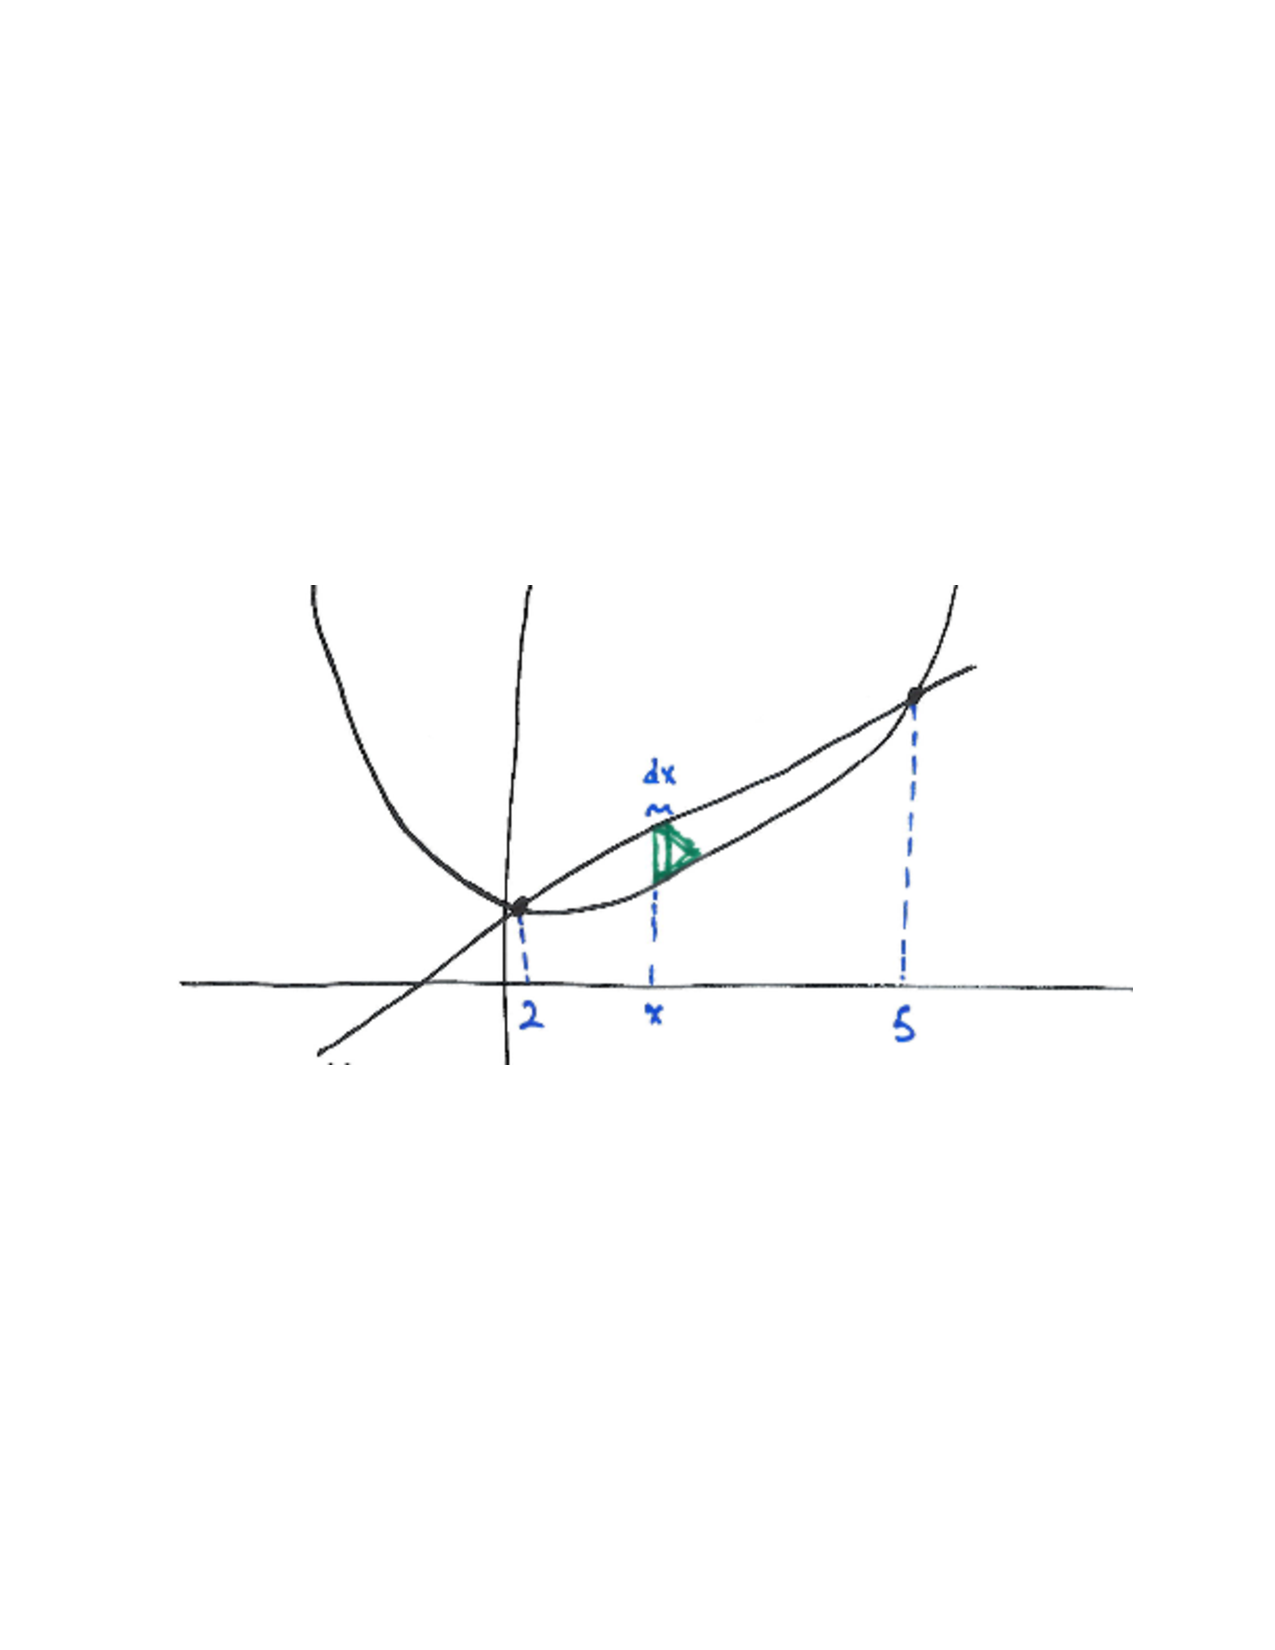
\includegraphics[trim= 170 270 150 280, scale=0.8]{Figure6-4-2.pdf}
		\end{image}

		{\bf Washers: }
		
		{\bf Shells: }
		\end{freeResponse}
		
		
		
		\item  $y=-4$  
		\begin{freeResponse}
		{\bf Washers: }
		
		{\bf Shells: }
		\end{freeResponse}
		
		
		
		\item  $y=22$
		\begin{freeResponse}
		{\bf Washers: }
		
		{\bf Shells: }
		\end{freeResponse}
		
		
		
		\item  the $y$-axis
		\begin{freeResponse}
		{\bf Washers: }
		
		{\bf Shells: }
		\end{freeResponse}
		
		
		
		\item  $x=-3$
		\begin{freeResponse}
		{\bf Washers: }
		
		{\bf Shells: }
		\end{freeResponse}
		
		
		
		\item$x=9$
		\begin{freeResponse}
		{\bf Washers: }
		
		{\bf Shells: }
		\end{freeResponse}
		
	\end{enumerate}
	
Use both the washer method as well as the shell method for each problem.  
Which method would you prefer for each problem?  Why?
	
\end{problem}

\begin{instructorNotes}
Split these between the groups.  
Allow 25 minutes for group work and 30 minutes for discussion.  
During the discussion, you might want to talk about all of the ``washer methods" before all of the ``shell methods".  
Be sure that they recognize (by the end) that we slice \dfn{perpendicular} to the axis of revolution in the washer method and \dfn{parallel} to the axis of revolution in the shell method.
\end{instructorNotes}







\begin{comment}
%problem 2
\begin{problem}

	\begin{freeResponse}
	
	\end{freeResponse}
		
\end{problem}

\begin{instructorNotes}

\end{instructorNotes}







%problem 3
\begin{problem}

	\begin{freeResponse}
	
	\end{freeResponse}

\end{problem}

\begin{instructorNotes}

\end{instructorNotes}
\end{comment}
















	
	
	
	
	
	
	
	
	

	










								
				
				
	














\end{document} 


















